% plots.tex — TikZ/pgfplots figures for hydrogen SDP results
%
% Compile: pdflatex plots.tex
% (requires data files in data/ from hydrogen_sdp.jl)

\documentclass[11pt,a4paper]{article}
\usepackage[margin=2cm]{geometry}
\usepackage{amsmath,amssymb}
\usepackage{pgfplots}
\pgfplotsset{compat=newest}
\usepgfplotslibrary{groupplots}
\usetikzlibrary{patterns}

\pgfplotsset{
    table/.append style={col sep=space, header=true},
}

\title{Barvinok--Pataki Numerical Verification:\\
       Hydrogen Atom in a Magnetic Field}
\author{Generated by \texttt{hydrogen\_sdp.jl} (Mosek solver)}
\date{}

\begin{document}
\maketitle

%% ========================================================================
%% Figure 1: Rank vs number of constraints (n=2, M=3/2)
%% ========================================================================

\begin{figure}[htbp]
\centering
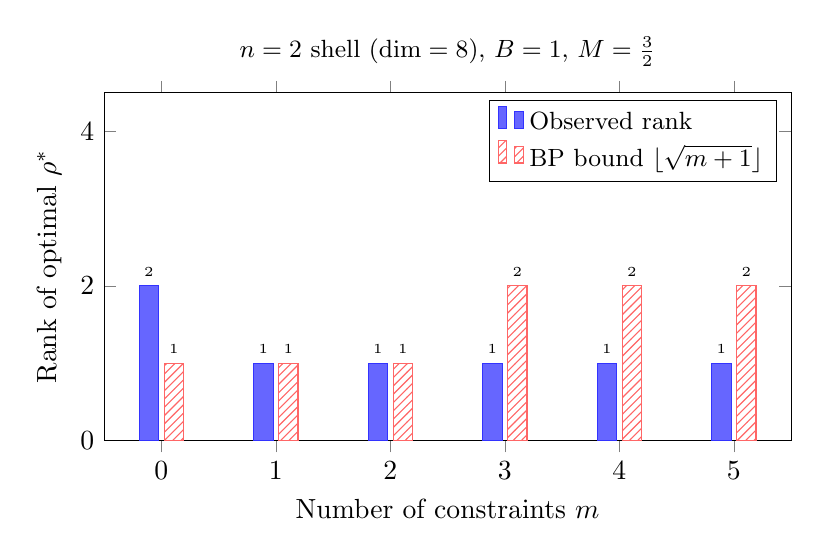
\begin{tikzpicture}
\begin{axis}[
    ybar,
    /pgf/bar width=7pt,
    width=0.85\textwidth,
    height=6cm,
    xlabel={Number of constraints $m$},
    ylabel={Rank of optimal $\rho^*$},
    ymin=0, ymax=4.5,
    xtick={0,1,2,3,4,5},
    legend style={at={(0.98,0.98)}, anchor=north east, font=\small},
    legend cell align=left,
    title={$n=2$ shell ($\dim=8$), $B=1$, $M=\tfrac{3}{2}$},
    title style={font=\small},
    nodes near coords,
    every node near coord/.append style={font=\tiny},
]

% Observed rank (from M=3/2 data)
\addplot[fill=blue!60, draw=blue!80] coordinates {
    (0, 2) (1, 1) (2, 1) (3, 1) (4, 1) (5, 1)
};

% BP bound floor(sqrt(m+1))
\addplot[fill=red!30, draw=red!60, pattern=north east lines, pattern color=red!60] coordinates {
    (0, 1) (1, 1) (2, 1) (3, 2) (4, 2) (5, 2)
};

\legend{Observed rank, BP bound $\lfloor\sqrt{m+1}\rfloor$}
\end{axis}
\end{tikzpicture}
\caption{Optimal rank vs.\ number of angular momentum constraints for
the $n=2$ hydrogen shell.  The Barvinok--Pataki bound
$r \leq \lfloor\sqrt{m+1}\rfloor$ is satisfied in all constrained
cases ($m \geq 1$).  At $m=0$ (unconstrained), the interior-point
solver finds the analytic centre (rank 2).}
\label{fig:rank-vs-m}
\end{figure}

%% ========================================================================
%% Figure 2: Optimal energy vs B for different constraint levels (n=3)
%% ========================================================================

\begin{figure}[htbp]
\centering
\begin{tikzpicture}
\begin{axis}[
    width=0.85\textwidth,
    height=7cm,
    xlabel={Magnetic field strength $B$ (units of $\mu_B B / \xi$)},
    ylabel={Optimal energy $E^*$ (units of $\xi$)},
    legend style={at={(0.02,0.98)}, anchor=north west, font=\small},
    legend cell align=left,
    title={Optimal energy vs.\ field strength ($n=3$ shell, $M=\tfrac{3}{2}$)},
    title style={font=\small},
    grid=major,
    grid style={gray!30},
]

\addplot[blue, thick, mark=none]
    table[x index=0, y index=2] {data/energy_vs_B_n3_m1.dat};
\addplot[red, thick, mark=none, dashed]
    table[x index=0, y index=2] {data/energy_vs_B_n3_m2.dat};
\addplot[green!60!black, thick, mark=none, dotted, line width=1.5pt]
    table[x index=0, y index=2] {data/energy_vs_B_n3_m3.dat};

\legend{$m=1$ ($J_z$ only), $m=2$ ($J_z + J^2$), $m=3$ ($J_z + J^2 + L^2$)}
\end{axis}
\end{tikzpicture}
\caption{Optimal energy as a function of magnetic field strength for
increasing numbers of constraints on the $n=3$ shell ($\dim=18$).
Adding constraints raises the minimum energy (the feasible set shrinks).
The $m=1$ curve shows the ground-state energy within the $m_j = 3/2$
sector, decreasing with $B$ due to the Zeeman splitting.  All optimizers
have rank $r = 1$ (pure states), consistent with the BP bound.}
\label{fig:energy-vs-B}
\end{figure}

%% ========================================================================
%% Figure 3: Leading eigenvalues of ρ* vs B (n=2, m=1 vs m=3, M=0.5)
%% ========================================================================

\begin{figure}[htbp]
\centering
\begin{tikzpicture}
\begin{groupplot}[
    group style={
        group size=2 by 1,
        horizontal sep=2cm,
    },
    width=0.48\textwidth,
    height=6.5cm,
    xlabel={$B$},
    ylabel={Eigenvalue of $\rho^*$},
    ymin=-0.05, ymax=1.1,
    grid=major,
    grid style={gray!30},
]

% Left: m=1 (pure throughout)
\nextgroupplot[
    title={$m=1$: $\langle J_z \rangle = \tfrac{1}{2}\hbar$},
    title style={font=\small},
    legend style={at={(0.98,0.55)}, anchor=east, font=\footnotesize},
]
\addplot[blue, thick, mark=none]
    table[x index=0, y index=4] {data/eigs_vs_B_n2_m1_M5.dat};
\addplot[red, thick, mark=none, dashed]
    table[x index=0, y index=5] {data/eigs_vs_B_n2_m1_M5.dat};
\addplot[green!60!black, thick, mark=none, dotted]
    table[x index=0, y index=6] {data/eigs_vs_B_n2_m1_M5.dat};
\legend{$\lambda_1$, $\lambda_2$, $\lambda_3$}

% Right: m=3 (could be rank 2 by BP)
\nextgroupplot[
    title={$m=3$: $\langle J_z \rangle, \langle J^2 \rangle, \langle L^2 \rangle$},
    title style={font=\small},
    legend style={at={(0.98,0.55)}, anchor=east, font=\footnotesize},
]
\addplot[blue, thick, mark=none]
    table[x index=0, y index=4] {data/eigs_vs_B_n2_m3_M5.dat};
\addplot[red, thick, mark=none, dashed]
    table[x index=0, y index=5] {data/eigs_vs_B_n2_m3_M5.dat};
\addplot[green!60!black, thick, mark=none, dotted]
    table[x index=0, y index=6] {data/eigs_vs_B_n2_m3_M5.dat};
\legend{$\lambda_1$, $\lambda_2$, $\lambda_3$}

\end{groupplot}
\end{tikzpicture}
\caption{Eigenvalue spectrum of the optimal $\rho^*$ as a function of
$B$ on the $n=2$ shell with $M = \tfrac{1}{2}$.
\textbf{Left:} $m=1$ (BP bound $r \leq 1$): the optimizer is pure
for all $B$.
\textbf{Right:} $m=3$ (BP bound $r \leq 2$): the three constraints
confine the optimizer.  The interior-point solver may find the
analytic centre (higher rank) rather than the extreme point.}
\label{fig:eigs-comparison}
\end{figure}

%% ========================================================================
%% Figure 4: Comparison of M=3/2 vs M=1/2 (rank behaviour)
%% ========================================================================

\begin{figure}[htbp]
\centering
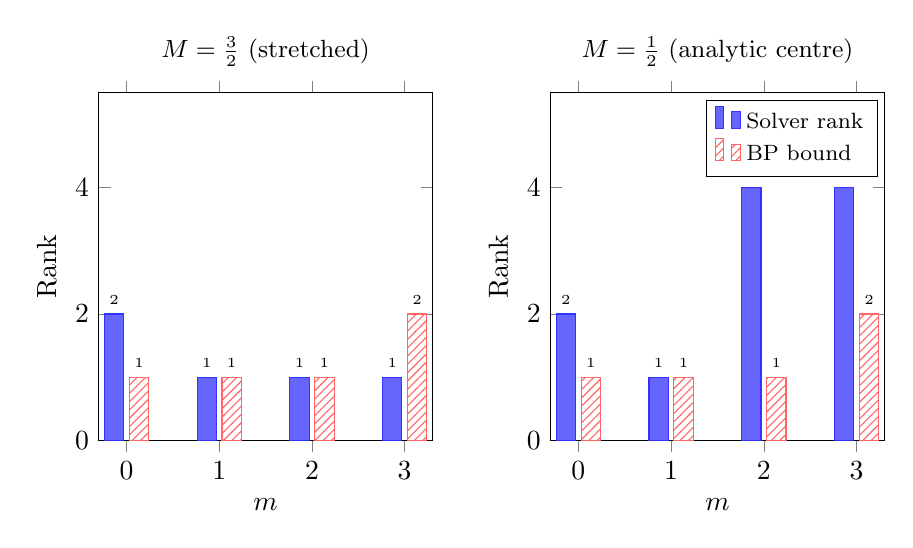
\begin{tikzpicture}
\begin{groupplot}[
    group style={
        group size=2 by 1,
        horizontal sep=1.5cm,
    },
    width=0.48\textwidth,
    height=6cm,
    ybar,
    /pgf/bar width=7pt,
    xlabel={$m$},
    ylabel={Rank},
    ymin=0, ymax=5.5,
    xtick={0,1,2,3},
    nodes near coords,
    every node near coord/.append style={font=\tiny},
]

% Left: M = 3/2 (stretched, pure throughout)
\nextgroupplot[title={$M = \tfrac{3}{2}$ (stretched)}, title style={font=\small}]
\addplot[fill=blue!60, draw=blue!80] coordinates {
    (0, 2) (1, 1) (2, 1) (3, 1)
};
\addplot[fill=red!30, draw=red!60, pattern=north east lines, pattern color=red!60] coordinates {
    (0, 1) (1, 1) (2, 1) (3, 2)
};

% Right: M = 1/2 (solver finds analytic centre)
\nextgroupplot[title={$M = \tfrac{1}{2}$ (analytic centre)}, title style={font=\small},
    legend style={at={(0.98,0.98)}, anchor=north east, font=\footnotesize},
    legend cell align=left]
\addplot[fill=blue!60, draw=blue!80] coordinates {
    (0, 2) (1, 1) (2, 4) (3, 4)
};
\addplot[fill=red!30, draw=red!60, pattern=north east lines, pattern color=red!60] coordinates {
    (0, 1) (1, 1) (2, 1) (3, 2)
};
\legend{Solver rank, BP bound}
\end{groupplot}
\end{tikzpicture}
\caption{Optimizer rank for the $n=2$ shell ($\dim = 8$).
\textbf{Left:} $M=\tfrac{3}{2}$ --- the optimizer is a unique
extreme point; rank satisfies BP bound.
\textbf{Right:} $M=\tfrac{1}{2}$ --- the optimal face is
degenerate; the interior-point solver converges to the analytic
centre with maximal rank on the optimal face.  Facial reduction
would recover an extreme point with rank $\leq\lfloor\sqrt{m+1}\rfloor$.}
\label{fig:M-comparison}
\end{figure}

%% ========================================================================
%% Figure 5: Rank vs Hilbert space dimension (scaling)
%% ========================================================================

\begin{figure}[htbp]
\centering
\begin{tikzpicture}
\begin{axis}[
    width=0.85\textwidth,
    height=6.5cm,
    xlabel={Hilbert space dimension $d = 2n^2$},
    ylabel={Rank of optimal $\rho^*$},
    ymin=0, ymax=55,
    xtick={8, 18, 32, 50},
    legend style={at={(0.02,0.98)}, anchor=north west, font=\small},
    legend cell align=left,
    title={Optimizer rank vs.\ Hilbert space dimension ($B=1$, $M=\tfrac{3}{2}$)},
    title style={font=\small},
    grid=major,
    grid style={gray!30},
]

% Observed ranks (all = 1)
\addplot[blue, thick, mark=*, mark size=3pt]
    table[x index=1, y index=3] {data/rank_vs_shell_m1.dat};
\addplot[red, thick, mark=square*, mark size=3pt]
    table[x index=1, y index=3] {data/rank_vs_shell_m2.dat};
\addplot[green!60!black, thick, mark=triangle*, mark size=3pt]
    table[x index=1, y index=3] {data/rank_vs_shell_m3.dat};

% Naive bound r ≤ d
\addplot[gray, dashed, thick, mark=none, domain=5:55, samples=2] {x};

% BP bounds (horizontal lines)
\addplot[blue!50, dotted, ultra thick, domain=5:55, samples=2] {1};
\addplot[green!60!black!50, dashdotted, thick, domain=5:55, samples=2] {2};

\legend{$m=1$, $m=2$, $m=3$,
        Na\"{\i}ve: $r \leq d$,
        BP ($m \leq 2$): $r \leq 1$,
        BP ($m = 3$): $r \leq 2$}
\end{axis}
\end{tikzpicture}
\caption{Optimizer rank as a function of Hilbert space dimension, for
$m = 1, 2, 3$ constraints.  The rank remains at 1 regardless of $d$,
in stark contrast to the na\"{\i}ve bound $r \leq d$ (dashed).
For the $n=5$ shell ($d = 50$), Barvinok--Pataki reduces the rank
bound from 50 to at most~2 (for $m=3$).}
\label{fig:rank-vs-dim}
\end{figure}

\end{document}
